\chapter{Interpretability and Case-Level Explanation}
\label{chap:explainability}

\section{Why Interpretability, and Why at Four Levels}

Chapter~\ref{chap:results} establishes that the HGT predicts more accurately than non-graph references and does so without identity shortcuts. A legal audience evaluates a prediction system on whether individual predictions can be \emph{read}, and on whether aggregate accuracy is explained by legally coherent structure.

This chapter treats the trained HGT as a \emph{frozen} object and dissects it through four lenses, each operating on the same artefacts (pre/post-GNN case embeddings, frozen graph, trained checkpoint) so results are directly comparable:

\begin{enumerate}
  \item \textbf{Representation level.} Does the GNN learn anything beyond input features? Probing classifier and t-SNE.
  \item \textbf{Component level.} Which node and edge types does the model depend on? Node-type zeroing and SHAP.
  \item \textbf{Error level.} Where does the representation fail? Decomposition by domain, statute density, facts length, year.
  \item \textbf{Case level.} For one prediction, why? \path{Graph_Analyser} produces, for a chosen case, the statutes, provisions, precedents, argument spans, and retrieved similar cases the frozen model used, verbalised through an LLM.
\end{enumerate}

The first three levels are global; the fourth is local. The bridge is the post-GNN case embedding: level~1 establishes that this embedding carries outcome-relevant structure; level~4 uses the same space to retrieve analogous training cases.

\section{Representation-Level Analysis}
\label{sec:repr_analysis}

\paragraph{Approach.} The frozen checkpoint is run over the full transductive graph and emits two case-level representations: the pre-GNN feature vector (1024-d \texttt{bge-m3} concatenated with scalar features, 1036-d total) and the post-GNN embedding (the 64-d \textsc{Case} representation). An L2-regularised logistic regression ($C=1$) is trained on each in turn, using the same train/test split as the main model.

\begin{table}[H]
  \centering
  \small
  \begin{adjustbox}{max width=\textwidth}
  \begin{tabular}{lccc}
    \toprule
    Probe input & Dim & Accuracy & Macro-F1 \\
    \midrule
    Majority-class baseline & $0$ & $0.6083$ & $0.3782$ \\
    Pre-GNN raw features    & $1036$ & $0.7443$ & $0.7372$ \\
    Post-GNN case embedding & $64$ & $0.7840$ & $0.7792$ \\
    \bottomrule
  \end{tabular}
  \end{adjustbox}
  \caption{Probing classifier on the cross-bucket fold-0 test split ($n=14{,}363$). Post-GNN is $+3.97$ points above pre-GNN despite being $16\times$ smaller --- the gain comes from \emph{information added by message passing}, not classifier capacity.}
  \label{tab:probing_results}
\end{table}

\begin{figure}[H]
  \centering
  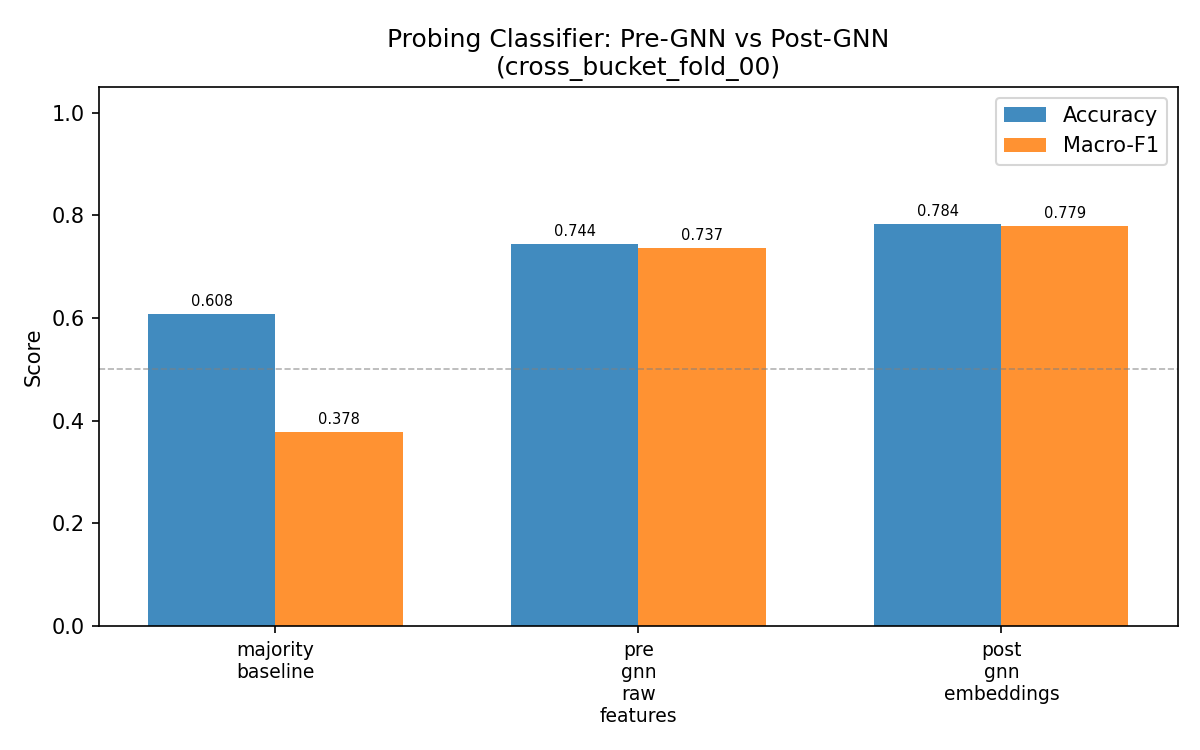
\includegraphics[width=0.65\linewidth]{figures/explainability/probing_bar.png}
  \caption{Probing accuracy at three stages. The gap between pre-GNN and post-GNN is the \emph{graph's} contribution.}
  \label{fig:probing_bar}
\end{figure}

The $+3.97$-point gap is the cleanest measurement of what message passing contributes: identical classifier, identical split, $16\times$ smaller representation. Holding the head fixed, the graph-propagated representation beats the text-only representation by a margin both statistically and operationally non-trivial.

\paragraph{Embedding geometry.} t-SNE projections of pre- and post-GNN embeddings, coloured by domain and by outcome label:

\begin{figure}[H]
  \centering
  \begin{minipage}{0.49\textwidth}
    {\footnotesize (a) Pre-GNN, by domain\par}
    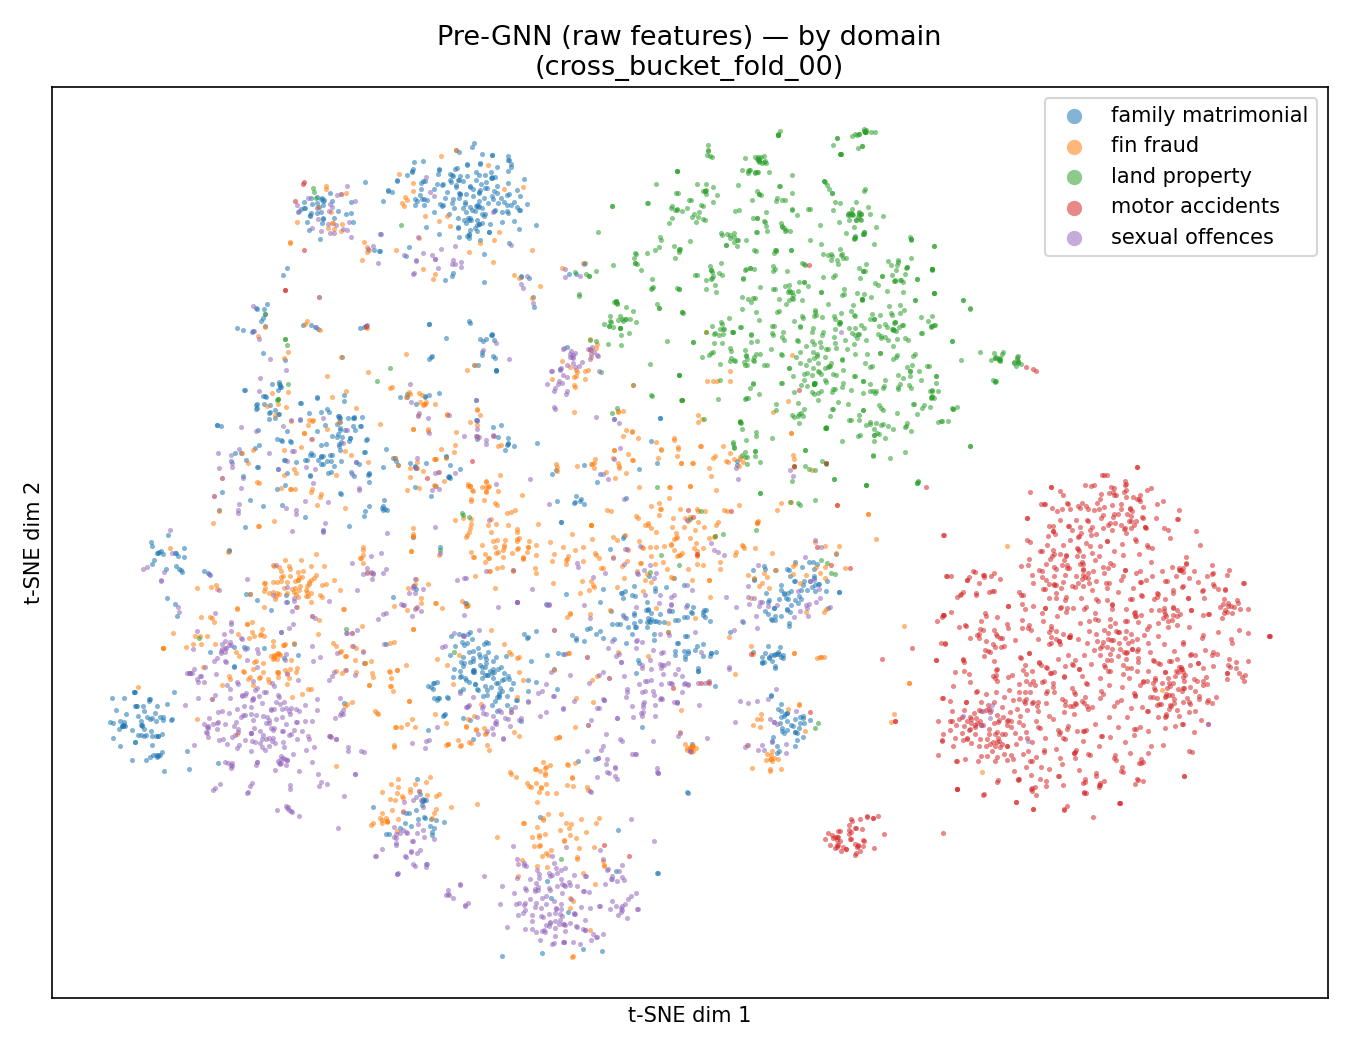
\includegraphics[width=\linewidth]{figures/explainability/tsne_pre_by_domain.png}
  \end{minipage}\hfill
  \begin{minipage}{0.49\textwidth}
    {\footnotesize (b) Post-GNN, by domain\par}
    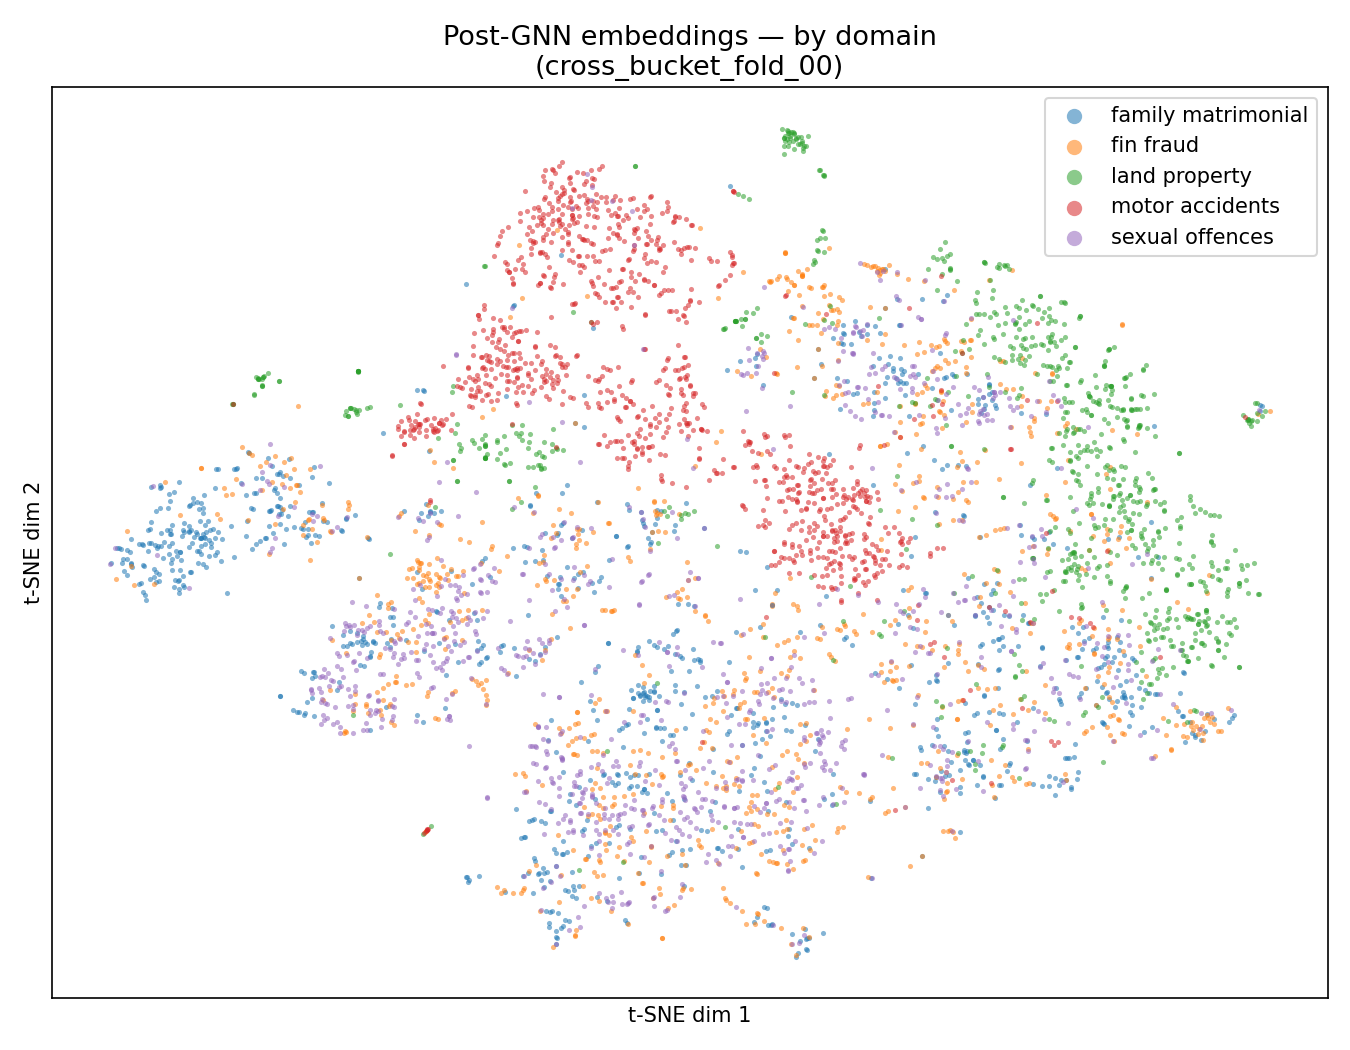
\includegraphics[width=\linewidth]{figures/explainability/tsne_post_by_domain.png}
  \end{minipage}

  \vspace{0.5em}

  \begin{minipage}{0.49\textwidth}
    {\footnotesize (c) Pre-GNN, by outcome\par}
    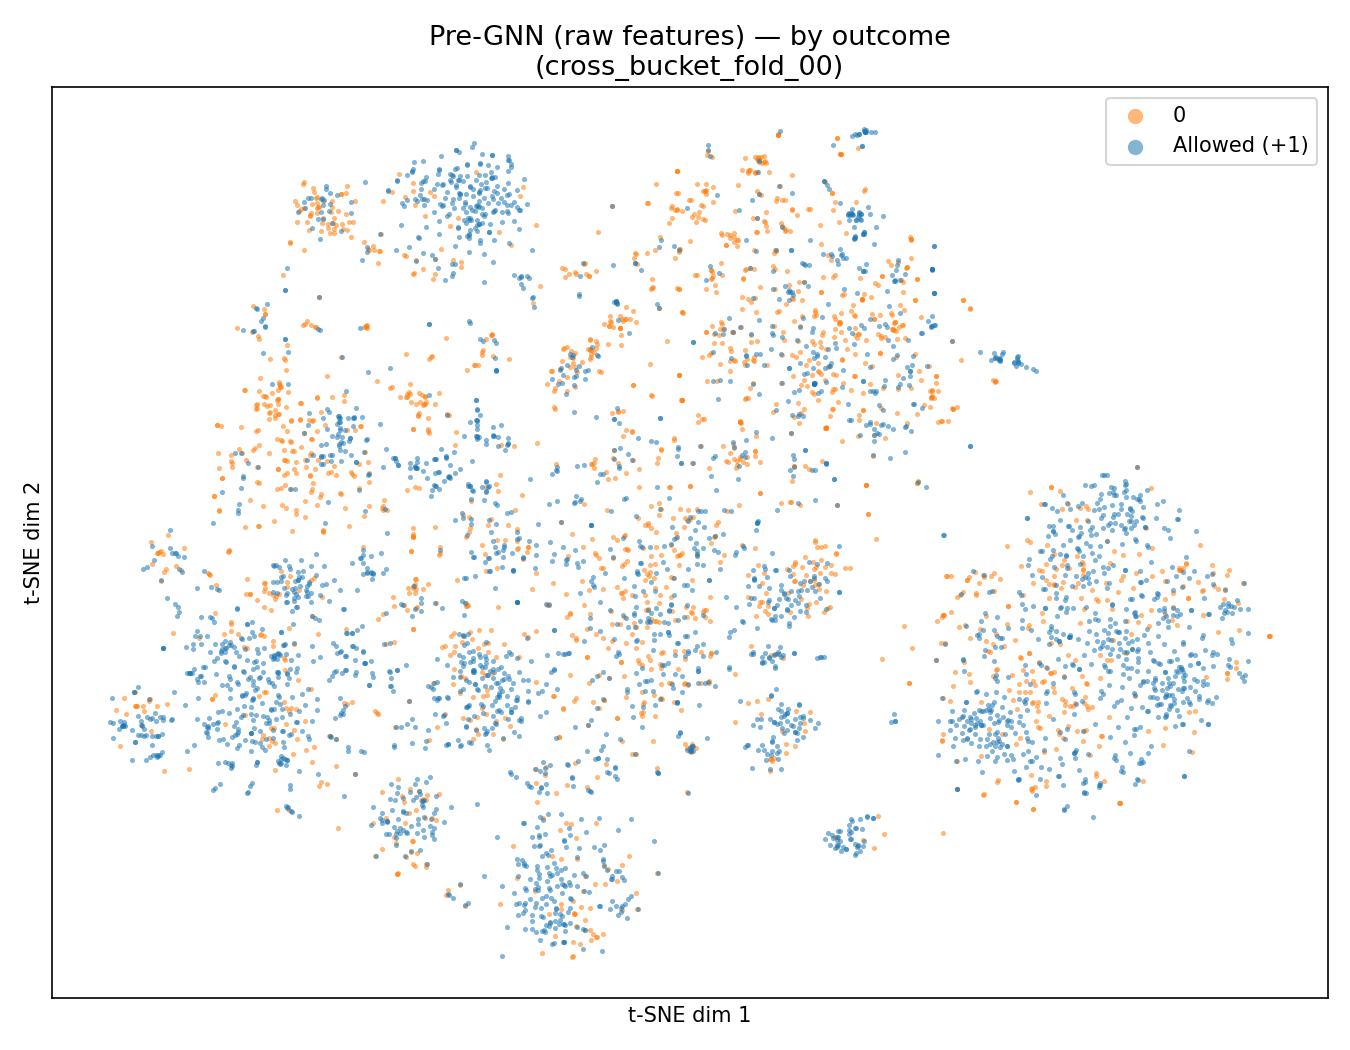
\includegraphics[width=\linewidth]{figures/explainability/tsne_pre_by_label.png}
  \end{minipage}\hfill
  \begin{minipage}{0.49\textwidth}
    {\footnotesize (d) Post-GNN, by outcome\par}
    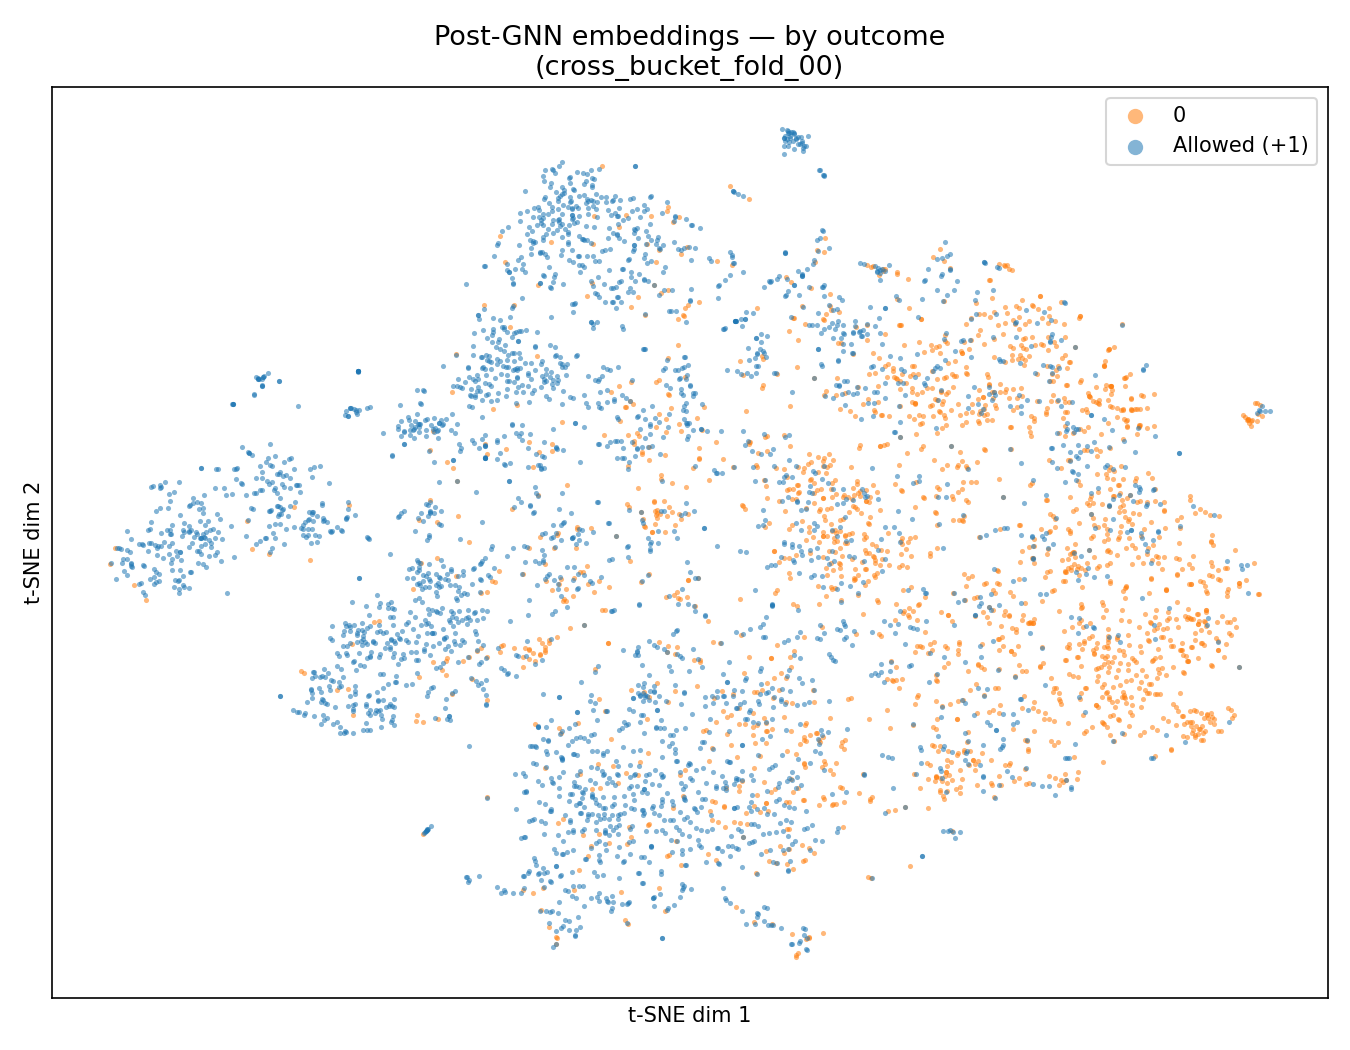
\includegraphics[width=\linewidth]{figures/explainability/tsne_post_by_label.png}
  \end{minipage}
  \caption{t-SNE projections of pre- and post-GNN case embeddings on fold~0. Domain structure is already present pre-GNN; label structure emerges only after graph propagation.}
  \label{fig:repr_tsne}
\end{figure}

Pre-GNN embeddings cluster strongly by \emph{domain}: \texttt{bge-m3} already separates the five buckets, but outcome labels are mixed within each cluster. Post-GNN preserves the domain clusters but reorganises each internally so outcome colour becomes visibly structured. The HGT's contribution is primarily \emph{within-domain} label geometry, not between-domain reorganisation.

\section{Component-Level Analysis}
\label{sec:component_analysis}

\paragraph{Node-type zeroing.} For each node type in turn, all features of that type are replaced with zeros and the frozen HGT is re-evaluated; the drop in test accuracy is the type's importance. Topology is preserved, isolating featural contribution.

\begin{figure}[H]
  \centering
  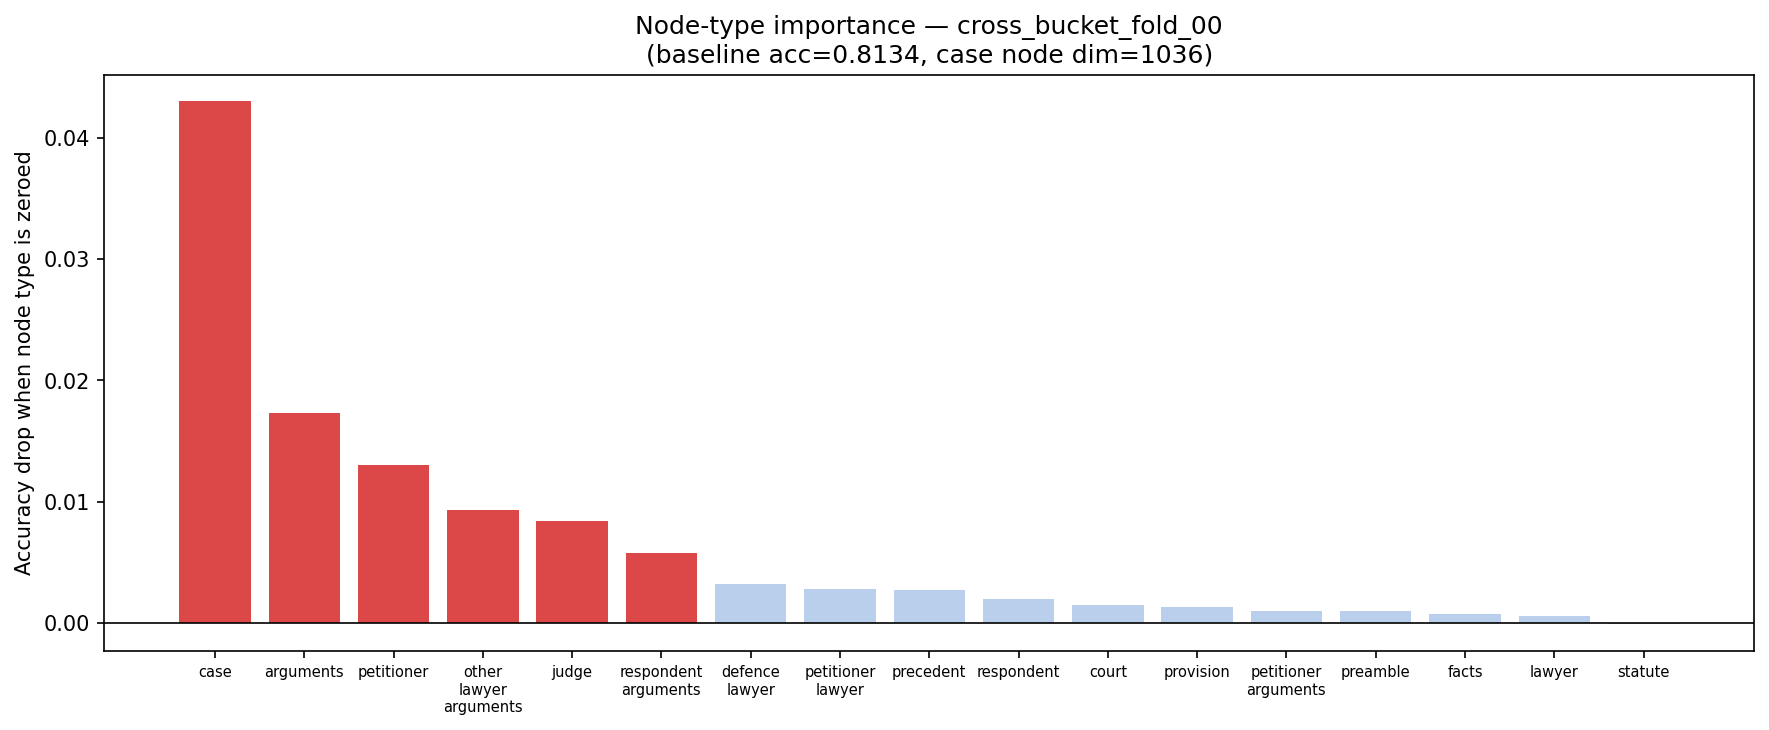
\includegraphics[width=0.78\linewidth]{figures/explainability/node_importance.png}
  \caption{Node-type importance via input zeroing on the cross-bucket baseline, fold~0. The \textsc{Case} node dominates, followed by argument-bearing text nodes and \textsc{Petitioner}/\textsc{Judge}.}
  \label{fig:node_importance}
\end{figure}

On the cross-bucket baseline (fold~0, baseline $0.8134$): \textsc{Case} ($-0.0430$) $\gg$ \textsc{Arguments} ($-0.0173$) $>$ \textsc{Petitioner} ($-0.0130$) $>$ \textsc{Other\_Lawyer\_Arguments} ($-0.0093$) $>$ \textsc{Judge} ($-0.0084$) $>$ \textsc{Respondent\_Arguments} ($-0.0058$) $>$ remaining types $\leq 0.0032$; statute zeroing is within noise of baseline.

Two readings. First, the model is anchored in the case node itself --- consistent with reading out from \textsc{Case}. Second, remaining signal is distributed across the argument stream and immediate participants rather than concentrated on any single authority type. Individual \textsc{Statute} and \textsc{Provision} nodes have near-zero per-type importance, so cross-case signal flows \emph{through the arguments} rather than directly through statutory features. Every top-tier component is a piece of graph-local legal context the \textsc{Case} node aggregates.

\paragraph{SHAP over the post-GNN embedding.} Mean absolute SHAP per dimension of the 64-d post-GNN embedding under a logistic-regression probe.

\begin{figure}[H]
  \centering
  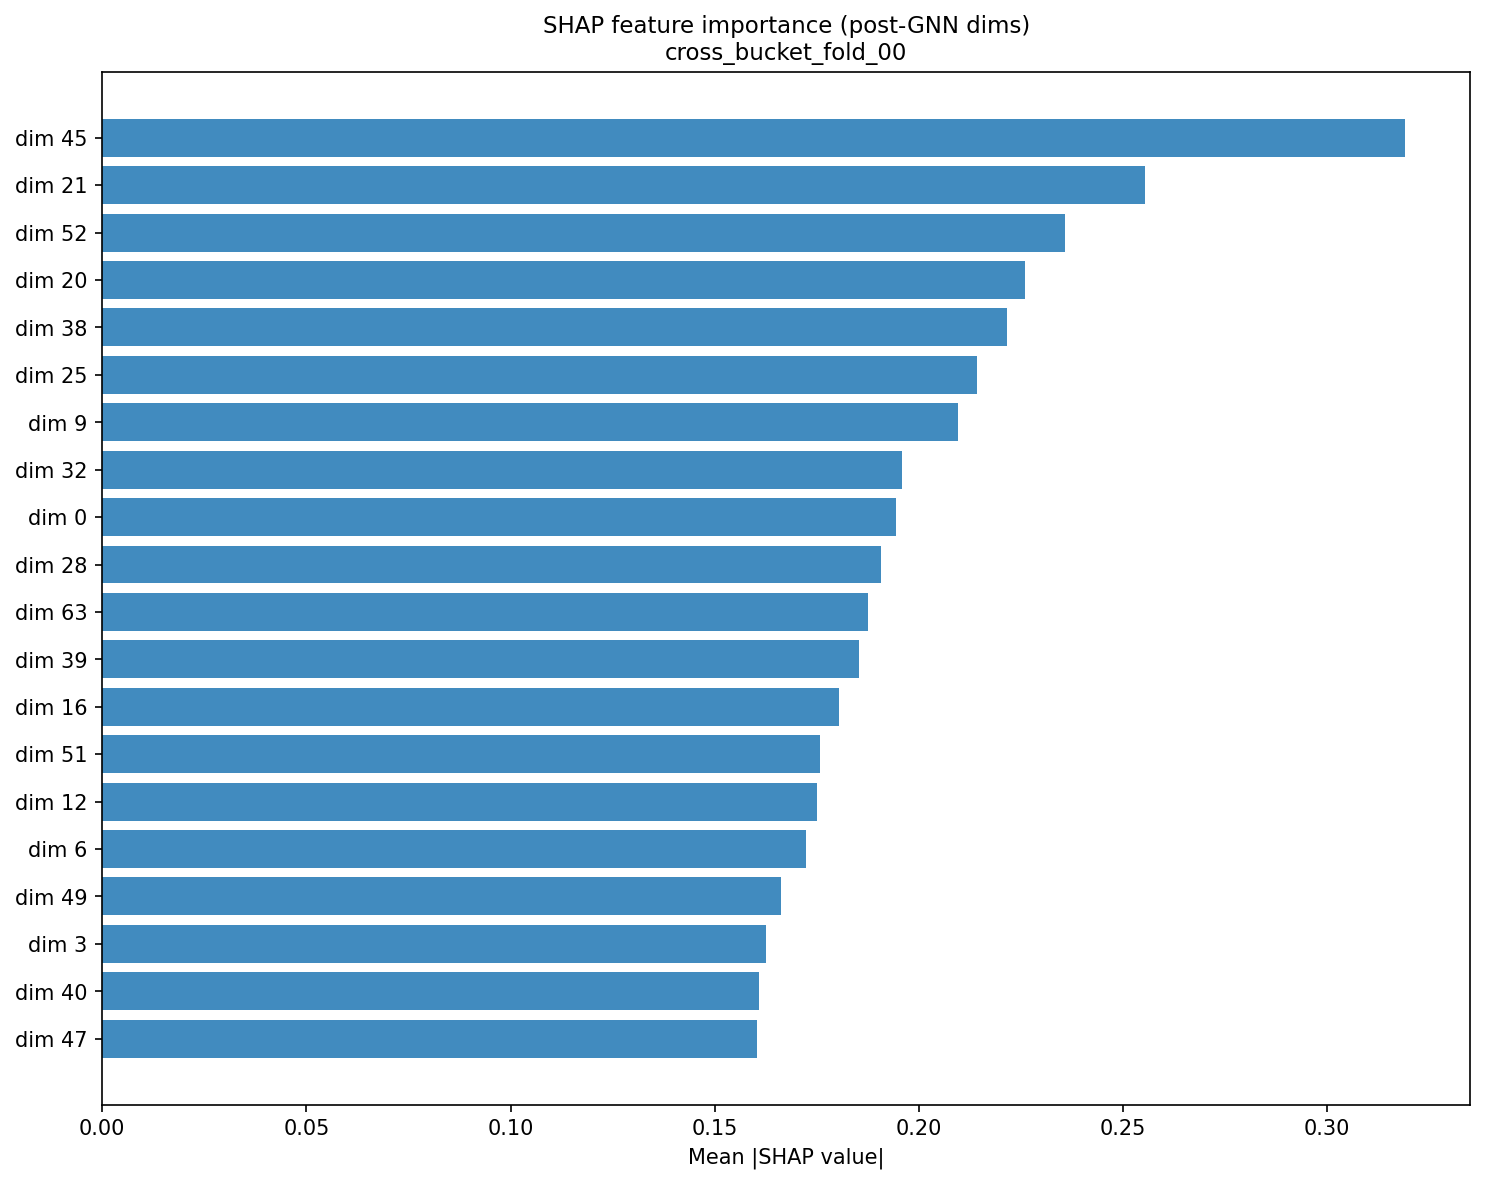
\includegraphics[width=0.78\linewidth]{figures/explainability/shap_bar.png}
  \caption{Mean absolute SHAP per latent dimension of the post-GNN embedding. Top six dimensions (\texttt{45, 21, 52, 20, 38, 25}) carry the largest contribution, but no single dimension dominates.}
  \label{fig:shap_bar}
\end{figure}

The remaining 58 dimensions still sum to a comparable share of the total mass. A distributed embedding is what one would want from a graph-level representation --- collapse onto a small number of dimensions would be evidence of a representational bottleneck. SHAP operates on the latent space, so it identifies important embedding \emph{dimensions}, not interpretable legal concepts; the case-level pipeline below is what produces legally named evidence.

\section{Error-Level Analysis}
\label{sec:error_analysis}

Test accuracy is decomposed along four orthogonal axes: legal domain, the number of statute nodes attached to a case (doctrinal density), \textsc{Facts} section length (narrative complexity), and judgment year (temporal drift).

\begin{figure}[H]
  \centering
  \begin{minipage}{0.49\textwidth}
    {\footnotesize (a) By domain\par}
    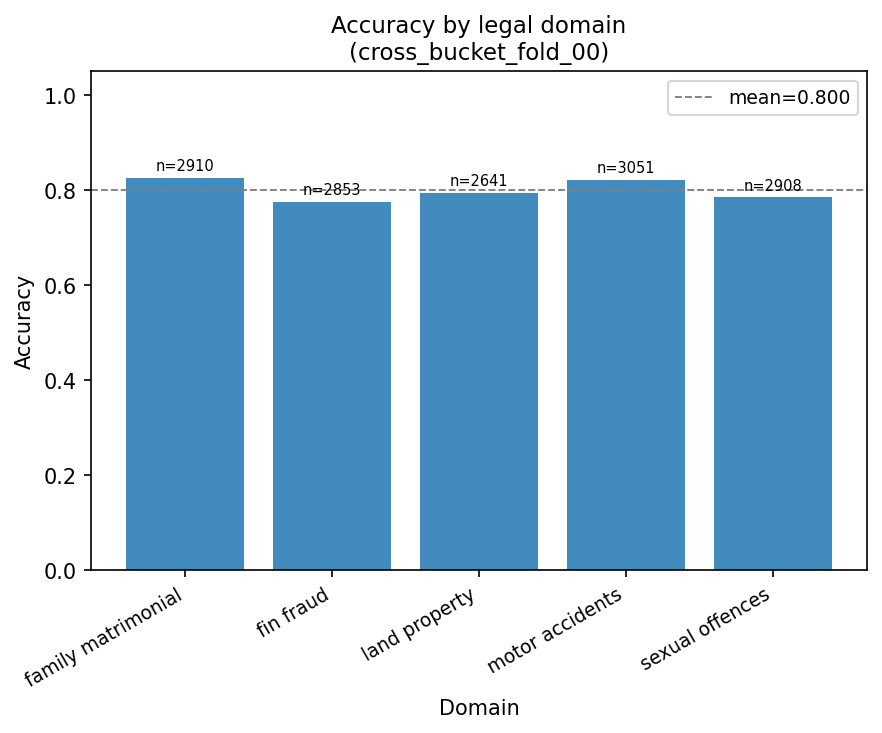
\includegraphics[width=\linewidth]{figures/explainability/error_by_domain.png}
  \end{minipage}\hfill
  \begin{minipage}{0.49\textwidth}
    {\footnotesize (b) By year\par}
    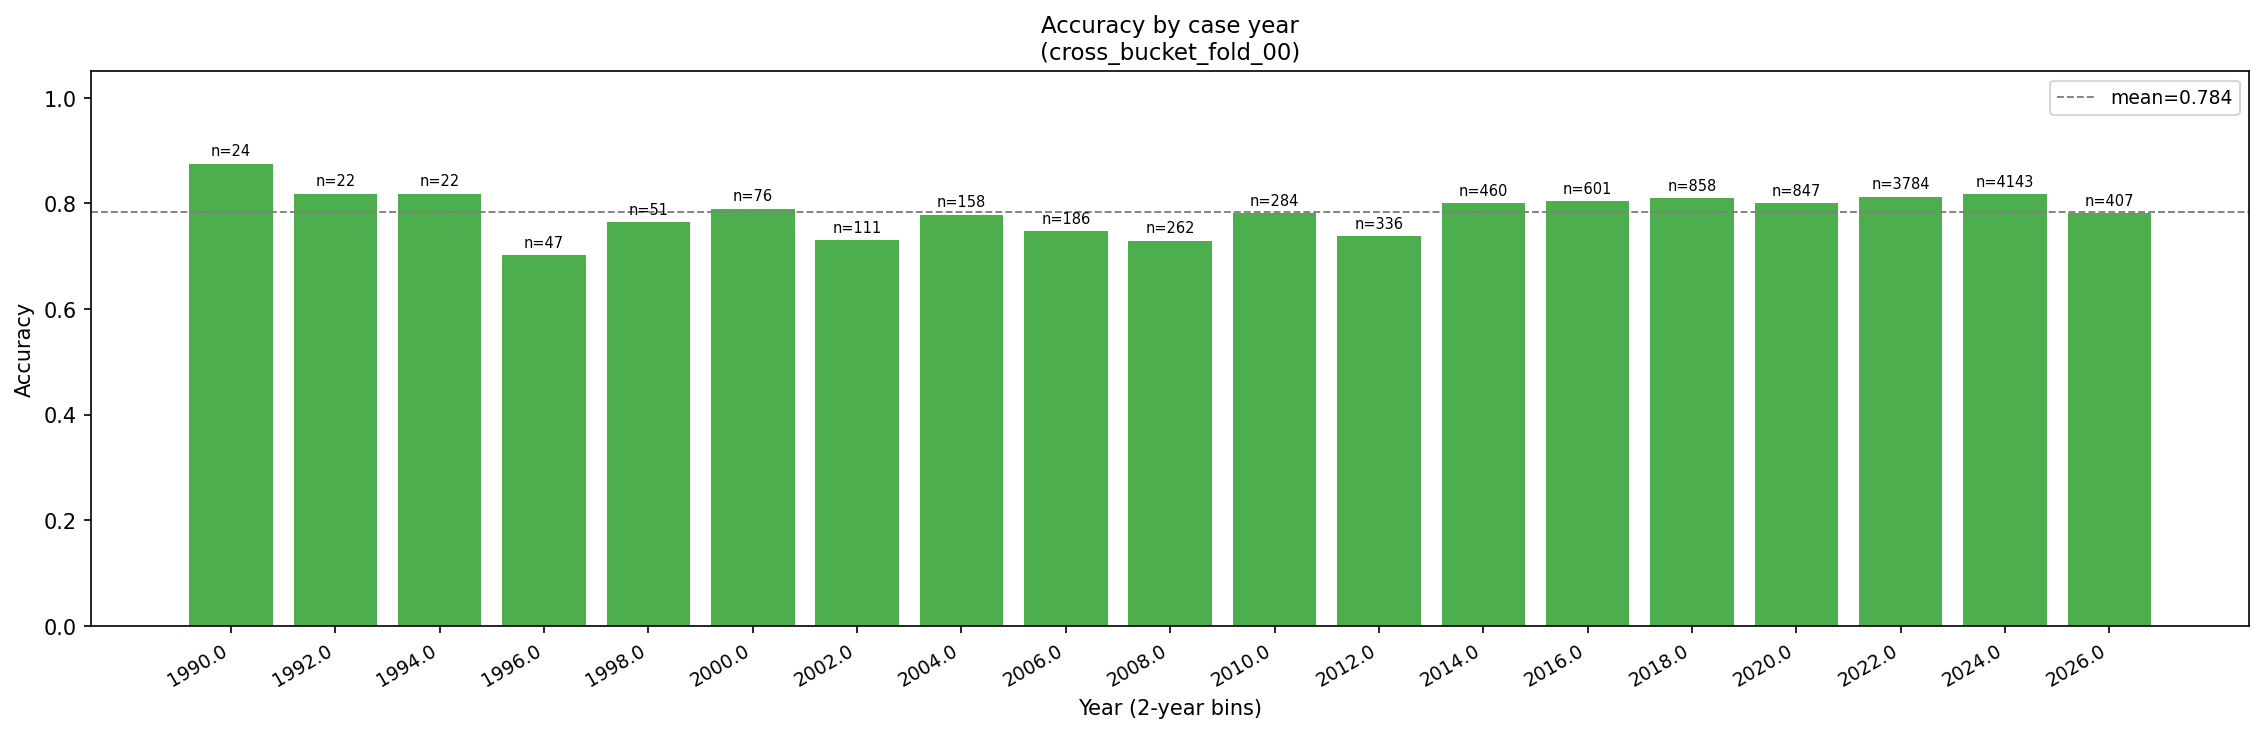
\includegraphics[width=\linewidth]{figures/explainability/error_by_year.png}
  \end{minipage}
  \caption{Error decomposition by legal domain and year. Year shows no systematic drift after small-$n$ early years are excluded.}
  \label{fig:error_domain_year}
\end{figure}

\begin{figure}[H]
  \centering
  \begin{minipage}{0.49\textwidth}
    {\footnotesize (a) By statute count\par}
    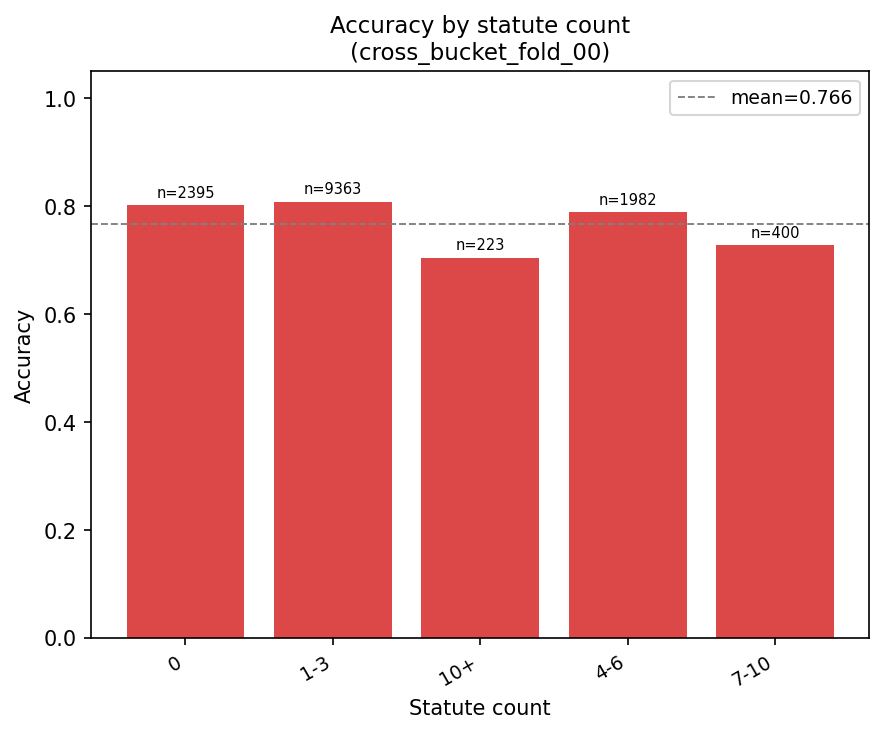
\includegraphics[width=\linewidth]{figures/explainability/error_by_statute.png}
  \end{minipage}\hfill
  \begin{minipage}{0.49\textwidth}
    {\footnotesize (b) By facts-length quintile\par}
    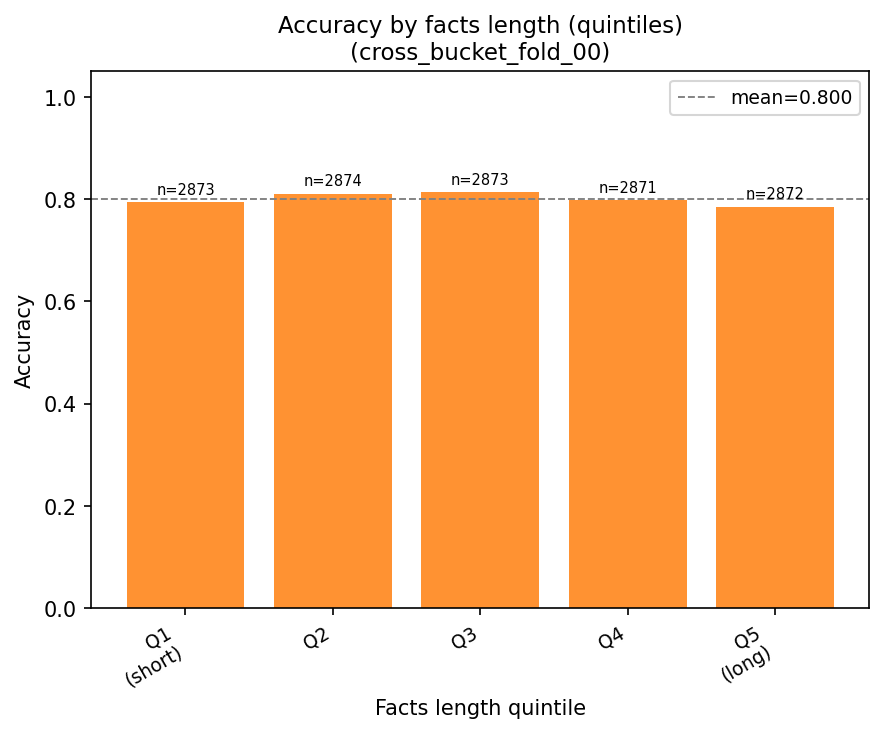
\includegraphics[width=\linewidth]{figures/explainability/error_by_facts_len.png}
  \end{minipage}
  \caption{Accuracy falls steadily on cases citing many statutes and on cases with the longest facts sections.}
  \label{fig:error_by_structure}
\end{figure}

\paragraph{Findings.}
\begin{itemize}
  \item \textbf{Domain ordering.} Overall fold-0 accuracy is $0.8005$. Family \& Matrimonial ($0.8254$) and Motor Accidents ($0.8209$) are strongest; Financial Fraud ($0.7757$) and Sexual Offences ($0.7844$) are weakest. Repetitive, highly-connected sub-graphs are easier to generalise over than doctrinally heterogeneous fraud and sexual-offence cases.
  \item \textbf{Doctrinal density hurts.} Accuracy falls from $\sim\!0.80$ on cases with 0--3 statute nodes to $0.7040$ on cases with $10+$. The model is better-behaved in single-frame disputes than in statutorily crowded judgments where several remedial pathways coexist.
  \item \textbf{Long narratives are slightly harder.} Longest-facts quintile $0.7852$ vs.\ $\sim\!0.81$ on the shortest. The decline is modest but monotone --- the failure pattern \texttt{hierarchical\_enc} was designed to mitigate.
  \item \textbf{Year is not a factor.} Per-year accuracy is flat, no temporal drift.
\end{itemize}

The global probes have answered the what, which, and where. They cannot answer the \emph{why} for individual predictions --- in particular, why a statute-dense case was misclassified, or why the confident-wrong predictions all look structurally plausible. That requires a case-scale pipeline.

\section{Case-Level Explanation}
\label{sec:case_pipeline}

For a specific test case, a legal user needs three things: a ranked set of \emph{legally named} entities (statutes, provisions, precedents, argument spans) the frozen model relied on; a short list of \emph{analogous training cases} that sit nearest in the model's representation space; and a natural-language synthesis a practitioner can read.

\path{Graph_Analyser} implements this as a five-phase pipeline over the frozen HGT. The bridge to the global analyses is the post-GNN embedding: Section~\ref{sec:repr_analysis} established that this embedding encodes outcome-relevant structure, so it is also the natural basis for retrieval-based case-level explanation.

\begin{table}[H]
  \centering
  \small
  \begin{adjustbox}{max width=\textwidth}
  \begin{tabular}{lll}
    \toprule
    Phase & Script & Primary outputs \\
    \midrule
    1--2: Inference + Index
      & \path{phase1_2_inference_and_index.py}
      & case embeddings, predictions, FAISS index over train split \\
    3: Explainer Training
      & \path{phase3_train_explainer.py}
      & trained heterogeneous PGExplainer \\
    4: Importance Extraction
      & \path{phase4_extract_importance.py}
      & per-case ranked statutes/provisions/precedents/arguments + similar cases \\
    5: LLM Translation
      & \path{phase5_llm_translate.py}
      & grounded natural-language narrative per case \\
    \bottomrule
  \end{tabular}
  \end{adjustbox}
  \caption{The five-phase \path{Graph_Analyser} pipeline.}
  \label{tab:explainer_pipeline}
\end{table}

Experiments use the cross-bucket pooled graph, fold~00 of the k-fold split (51{,}705 train, 5{,}745 val, 14{,}363 test), with the best \texttt{party\_args\_lr\_decay} HGT.

\paragraph{Phase 1--2: Frozen inference and retrieval index.} The frozen HGT runs in inference mode over the full graph and emits, per case node, the 64-d post-GNN embedding plus predicted label and per-class probabilities. A FAISS cosine-similarity index is built over the training-split embeddings only. Using the post-GNN embedding (rather than raw text or an earlier layer) is deliberate: neighbours returned are similar \emph{in the sense that matters for the frozen model's prediction}, making them legitimate explanatory analogues.

\paragraph{Phase 3: Heterogeneous PGExplainer.} The textbook approach is PGExplainer~\cite{luo2020parameterized}, but PyG's implementation is homogeneous: it weights messages via \texttt{edge\_weight}, which HGTConv does not accept. Our adaptation (\path{analyser/hetero_pg_explainer.py}) keeps the PGExplainer objective but changes the mask semantics: rather than weighting messages, the explainer selects which edges \emph{exist}. Given a binary edge mask produced by a shared MLP that ingests source/destination embeddings and a relation-type embedding, the masked edges are removed from \texttt{edge\_index\_dict} and the frozen HGT is rerun on the reduced graph. The mask is relaxed via Gumbel-sigmoid straight-through estimation.

Three loss terms: (i) cross-entropy between the masked-graph and full-graph predictions; (ii) $\ell_1$ size penalty for sparse explanations; (iii) entropy penalty preventing convergence to uniform weights. Temperature is annealed from $5$ to $1$ over 30 epochs.

\paragraph{Phase 4: From edge scores to legal evidence.} Edge importance is computed once globally rather than per-case: the trained explainer's edge-score function is evaluated on every edge, and each case's explanation is assembled from the scores reachable from the target. For each case: (i) the $k$-hop subgraph is collected by undirected BFS with depth matching the two HGT layers; (ii) edge scores are restricted to incident edges; (iii) edge scores aggregate to node importance via the max-incident-edge rule, ranked by type into top-$N$ lists for \textsc{Statute}, \textsc{Provision}, \textsc{Precedent}, and the four argument-node variants; (iv) the FAISS index is queried with the target's post-GNN embedding to retrieve the top-$k$ training cases ($k=3$ default), with their labels and argument-context snippets.

\paragraph{Phase 5: LLM translation.} The Phase~4 record is fed to a Mistral-Small~24B model running locally under vLLM, with a prompt that produces a structured narrative covering the predicted outcome, governing statutes, key provisions, retrieved analogous precedents, argument patterns, and a plain-language reasoning summary.

The LLM is not an open-ended legal reasoner: it receives \emph{only} the evidence bundle plus the pre-outcome textual content (preamble and arguments). The true outcome is surfaced as an ``actual outcome (for reference)'' field so the narrative can flag model errors rather than silently rationalise them, but the LLM is instructed to explain the \emph{predicted} label. Evidence selection is done by the trained explainer; verbalisation by the LLM. This boundary is what makes the narrative attributable to the HGT's behaviour rather than to LLM priors.

\section{A Worked Example: A Confidently-Correct Case}
\label{sec:worked_correct}

Test case 10212 (\emph{Sanjeev Kumar vs State of Punjab and Another}, 2023). The HGT predicts \emph{petitioner wins} with probability $0.9998$; ground truth is also \emph{petitioner wins}.

\begin{figure}[H]
  \centering
  \begin{minipage}{0.49\textwidth}
    {\footnotesize (a) Target in post-GNN t-SNE space\par}
    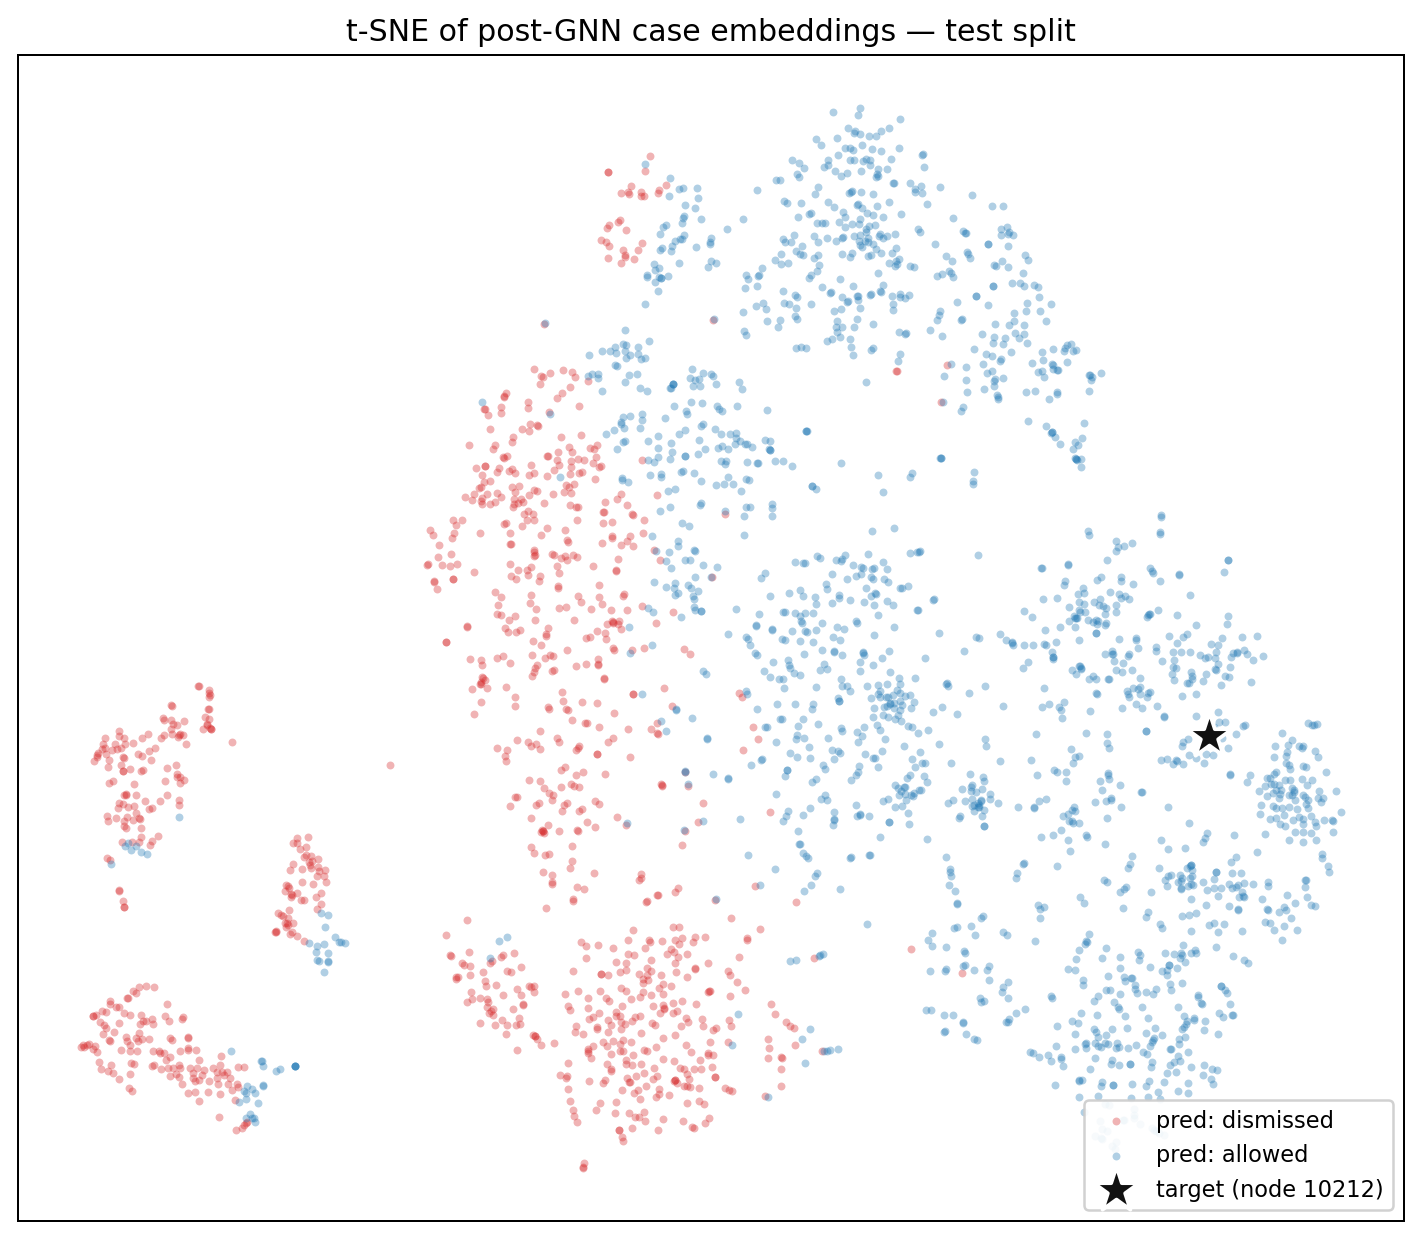
\includegraphics[width=\linewidth]{figures/explainability/correct_10212_panel_a_tsne.png}
  \end{minipage}\hfill
  \begin{minipage}{0.49\textwidth}
    {\footnotesize (b) Top evidence subgraph\par}
    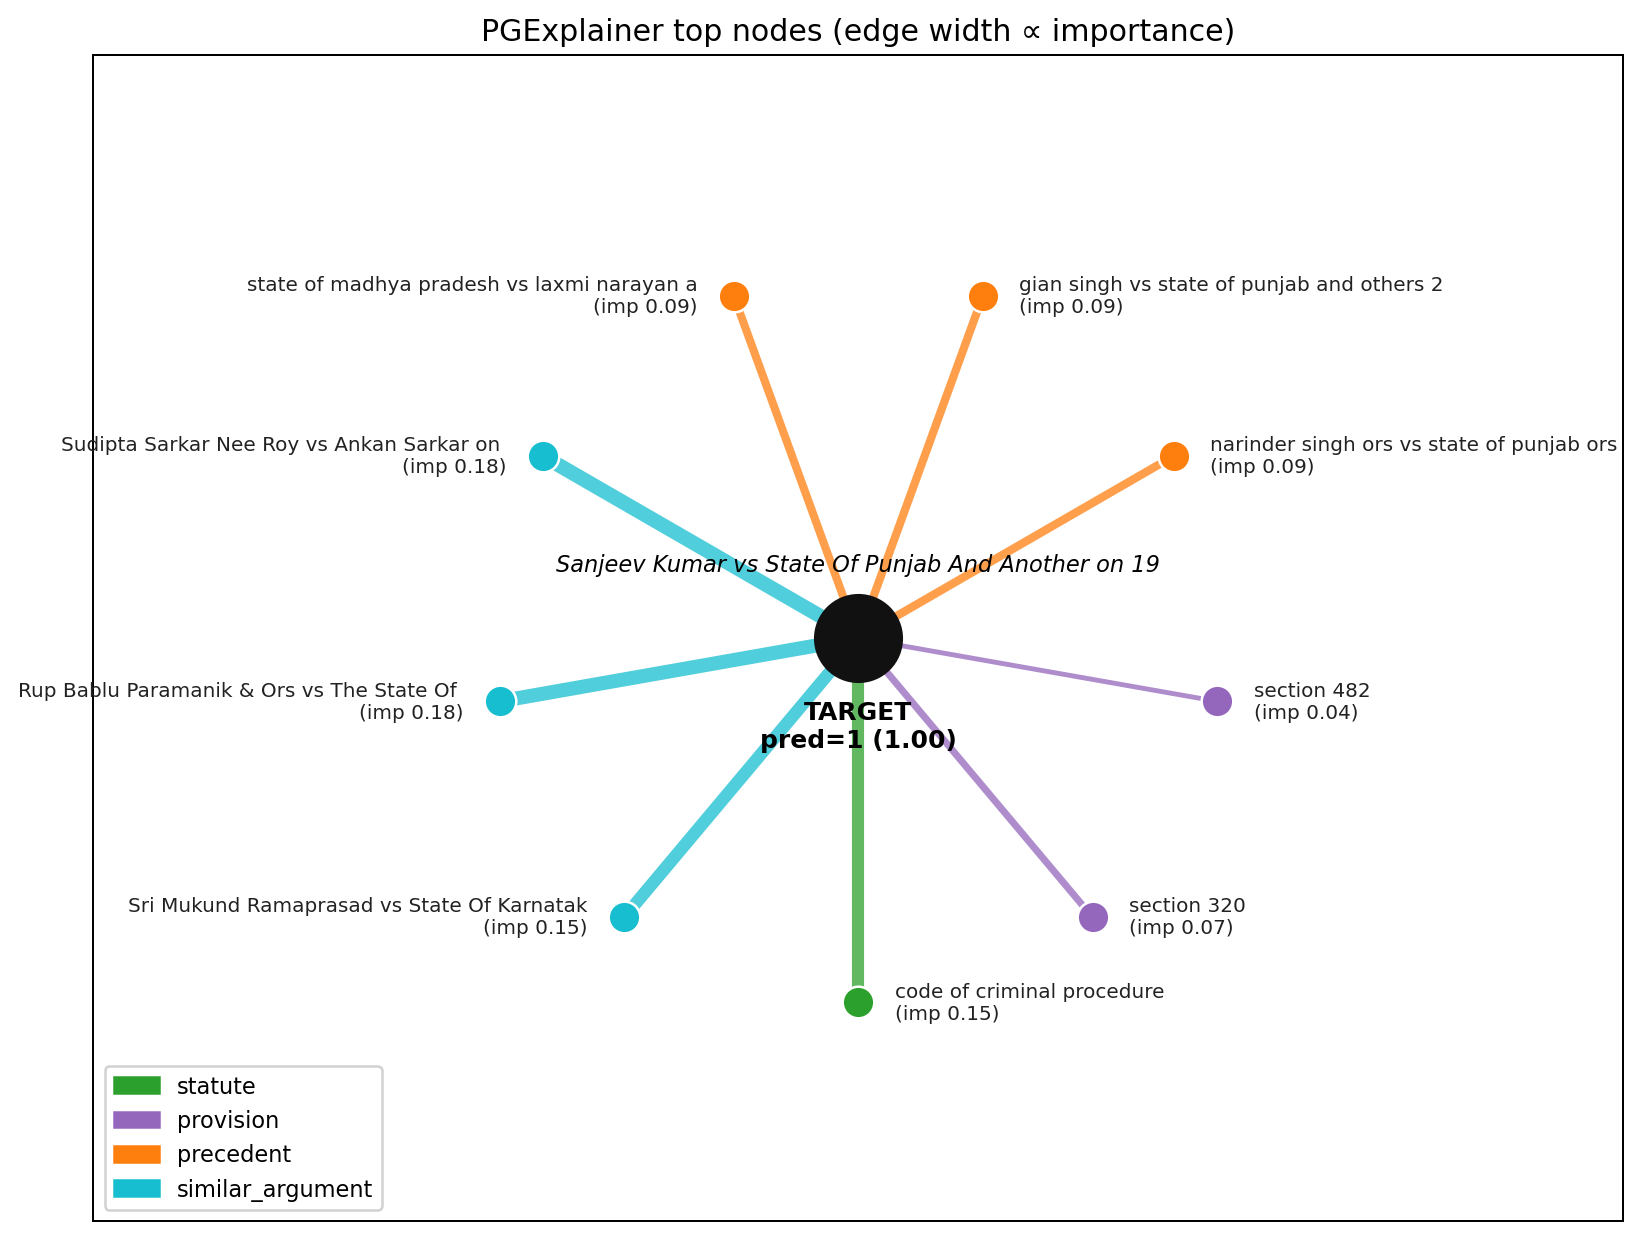
\includegraphics[width=\linewidth]{figures/explainability/correct_10212_panel_b_subgraph.png}
  \end{minipage}
  \caption{Confidently-correct case 10212. (a) location in post-GNN space; (b) top-weighted statutes, provisions, precedents, and arguments.}
  \label{fig:case_correct}
\end{figure}

The governing statute surfaced is the \emph{Code of Criminal Procedure}; the top two provisions are Section~320 CrPC (compounding of offences) and Section~482 CrPC (inherent power of the High Court to quash) --- exactly the doctrinal pair underlying the family-matrimonial ``quash-on-compromise'' pattern. The top retrieved analogues --- \emph{Gurmail Singh}, \emph{Satinder Pal Verma}, \emph{Ravi Kumar Prashar} v.\ State of Punjab --- are all allowed, with cosine similarity $>\!0.99$ in post-GNN space.

The Phase~5 narrative reconstructs this as standard quash-on-compromise reasoning: the parties have settled; Section~320 CrPC governs compounding; Section~482 CrPC authorises the High Court to quash; \emph{Gian Singh v.\ State of Punjab} (2012) and \emph{State of MP v.\ Laxmi Narayan} (2019) establish that inherent-power quashing is available even for non-compoundable offences when the compromise is genuine. Every named statute, provision, and precedent comes from the Phase~4 evidence bundle; the LLM supplies the connective tissue.

\section{When Confidence and Correctness Diverge}
\label{sec:right_vs_wrong}

The interesting failures are not low-confidence mistakes (those are honest and reflected in calibration) but \emph{high-confidence} mistakes. The retrieval framing provides a natural diagnostic: compare the predicted-class label of the top-$k$ retrieved neighbours with the true label.

\paragraph{Aggregate.} Of test cases with predicted-class probability $>\!0.99$, 1{,}460 are \emph{confidently correct}; 72 are \emph{confidently wrong}. For the wrong subset, the mean fraction of top-$5$ neighbours matching the \emph{predicted} (incorrect) label is $0.989$; for the \emph{true} label, $0.011$. 68 of the 72 have all five top neighbours from the predicted class.

\begin{figure}[H]
  \centering
  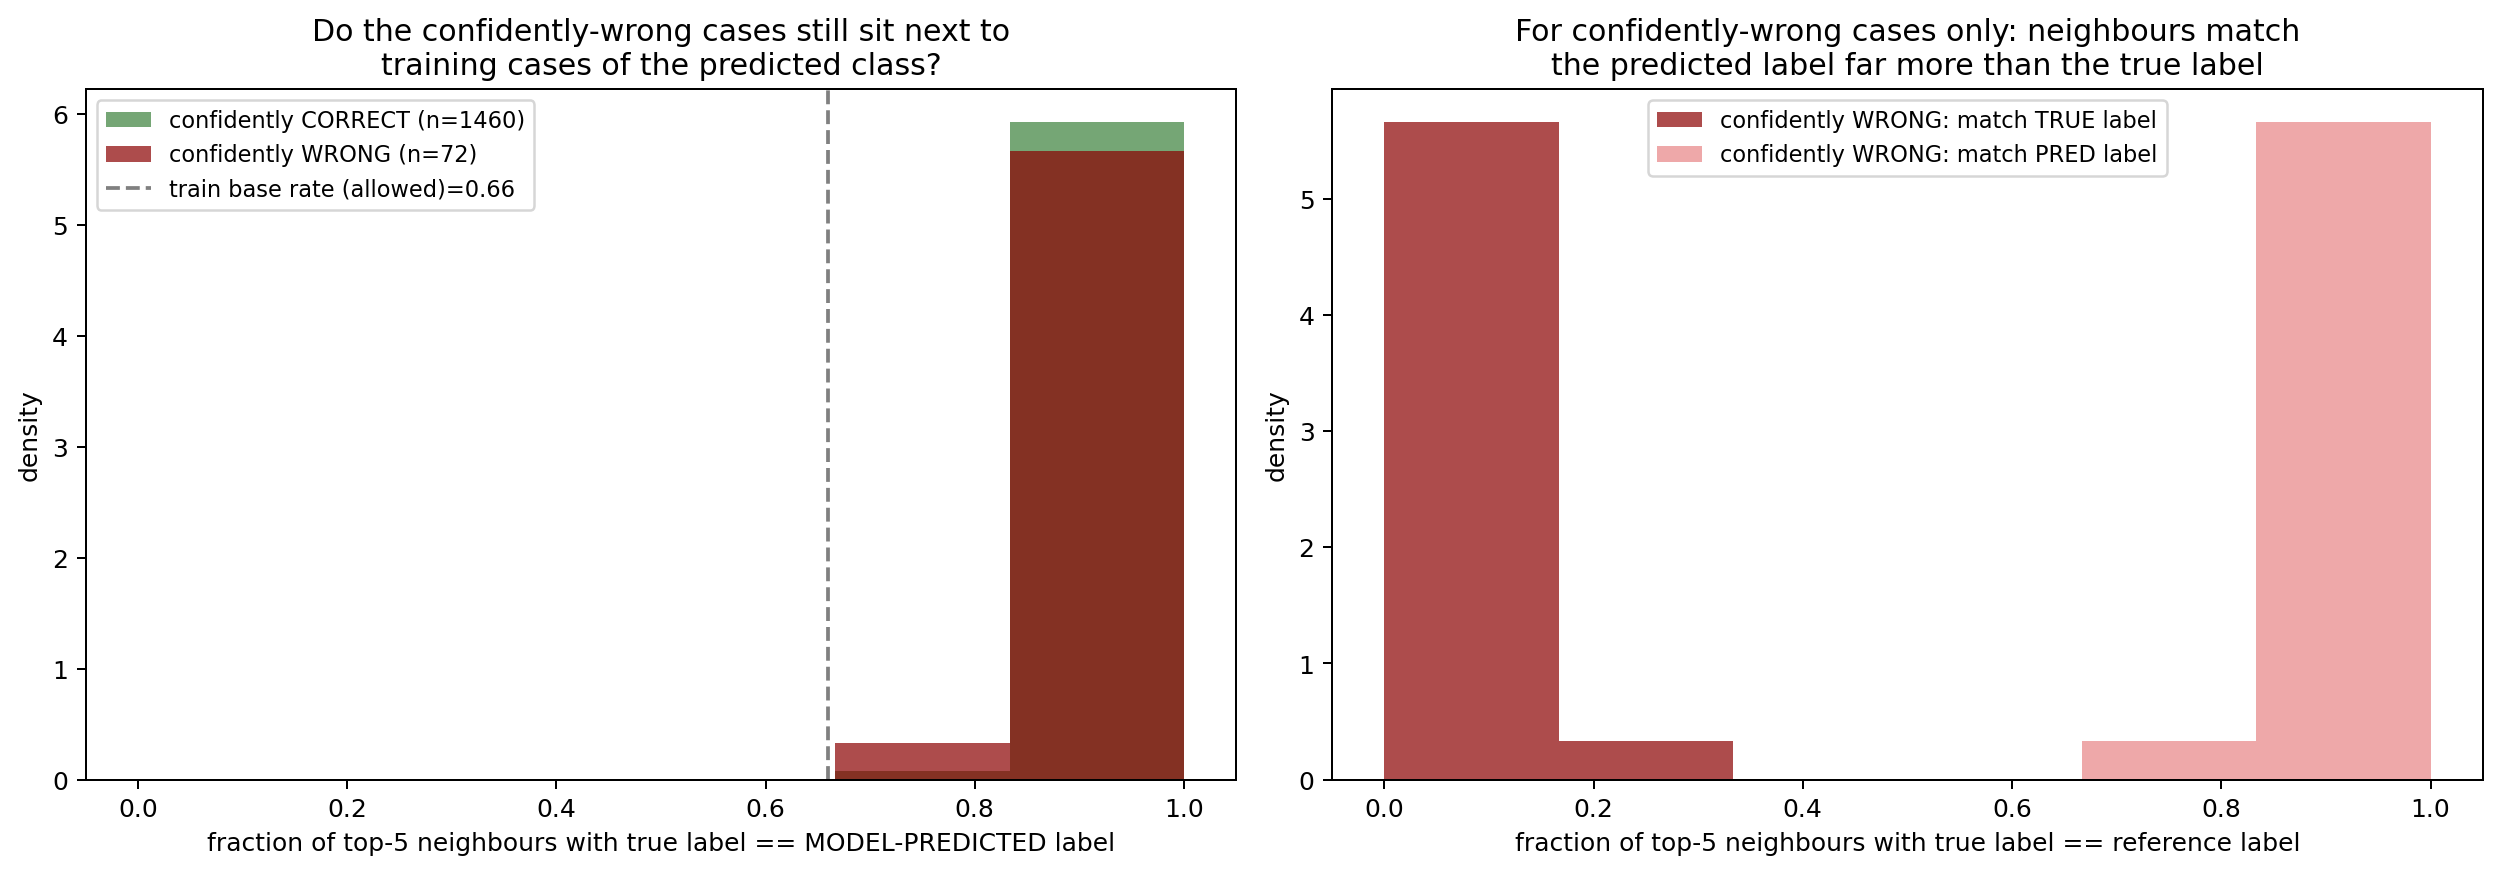
\includegraphics[width=0.78\linewidth]{figures/explainability/neighbour_alignment_hist.png}
  \caption{Distribution of neighbour-label alignment for high-confidence predictions. Confidently-correct cases: top-5 neighbours match the true label. Confidently-wrong cases: neighbours match the \emph{predicted} label and disagree with truth.}
  \label{fig:neighbour_alignment}
\end{figure}

Confident errors are not random: they occur when the post-GNN embedding places the target inside the wrong outcome neighbourhood, causing both the prediction and the retrieval-based explanation to reinforce the same mistaken structure. This is sharper than ``the model is uncertain''. The very mechanism used to explain successes also amplifies confident errors --- an argument for pairing the prediction with a class-boundary proximity score at deployment time, rather than classifier confidence alone.

\paragraph{Worked confident-wrong example.} Case 13701 (\emph{Umesh V vs State of Kerala}, 2023). Predicted \emph{petitioner wins} at $0.9998$; true label \emph{petitioner loses}. All three displayed neighbours --- \emph{Faisal P.C.}, \emph{Nisamudheen M.M.}, \emph{Nithin Antony} v.\ State of Kerala, filed on adjacent days --- are wins, each with cosine similarity $>\!0.98$.

\begin{figure}[H]
  \centering
  \begin{minipage}{0.49\textwidth}
    {\footnotesize (a) Target in post-GNN t-SNE\par}
    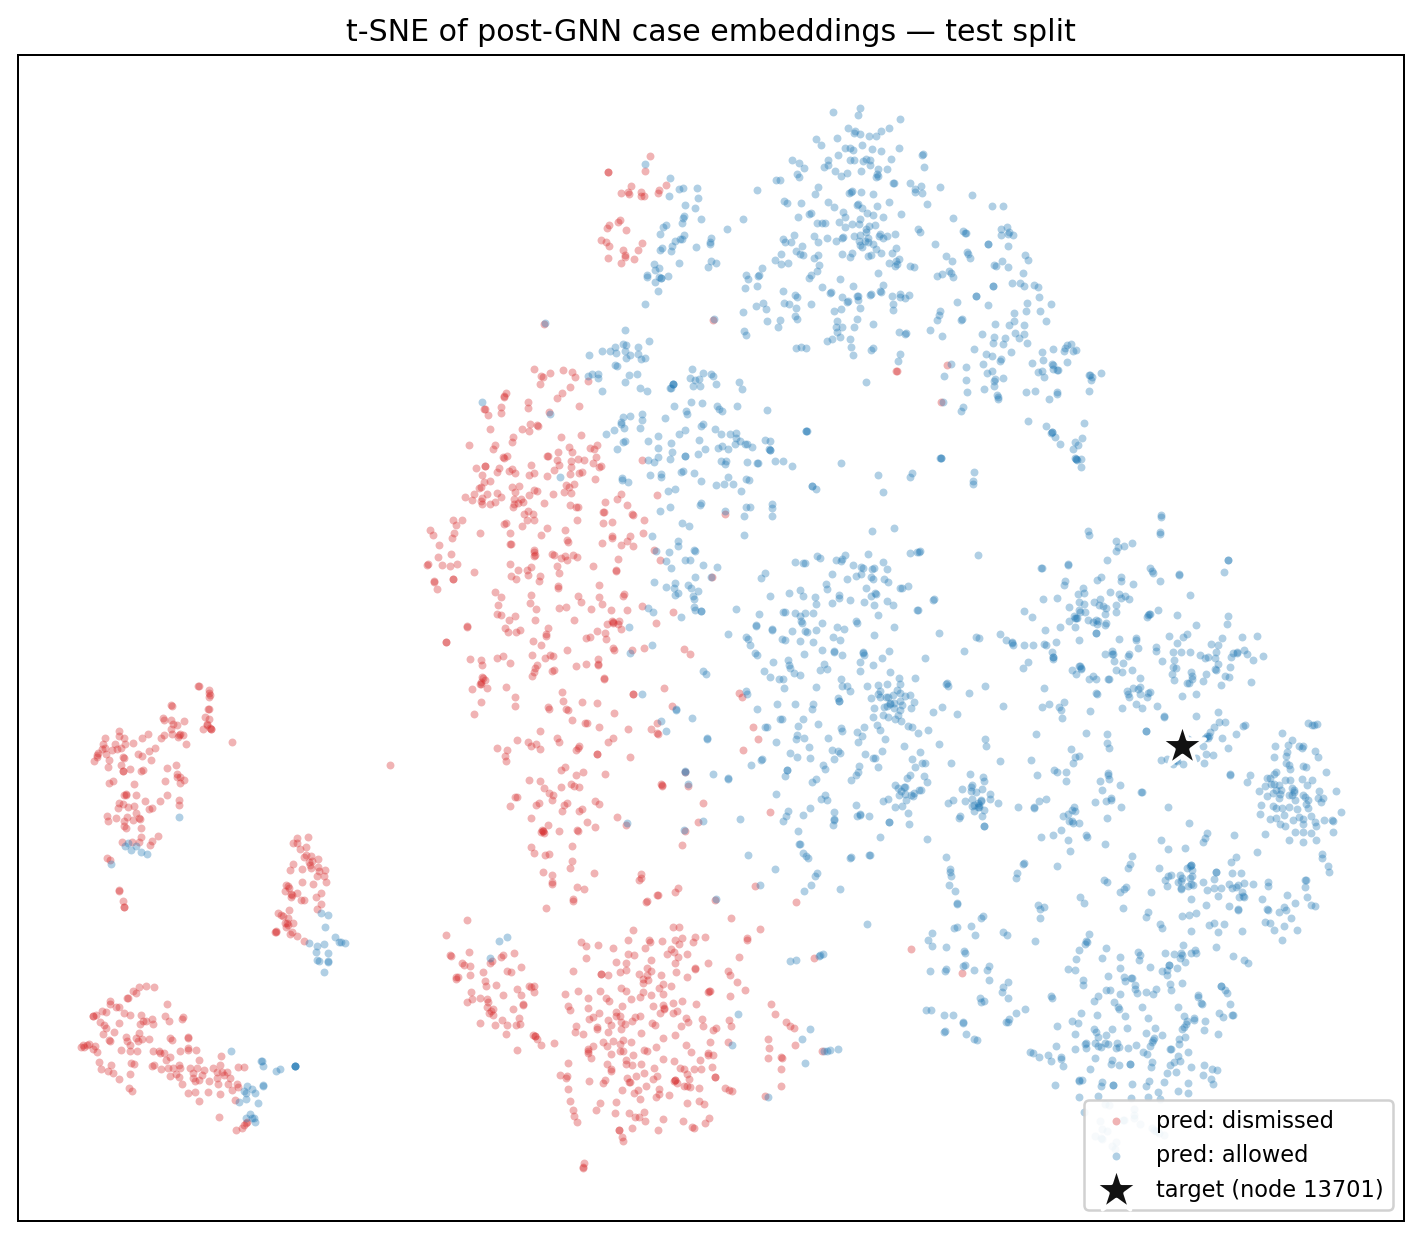
\includegraphics[width=\linewidth]{figures/explainability/wrong_13701_panel_a_tsne.png}
  \end{minipage}\hfill
  \begin{minipage}{0.49\textwidth}
    {\footnotesize (b) Top evidence subgraph\par}
    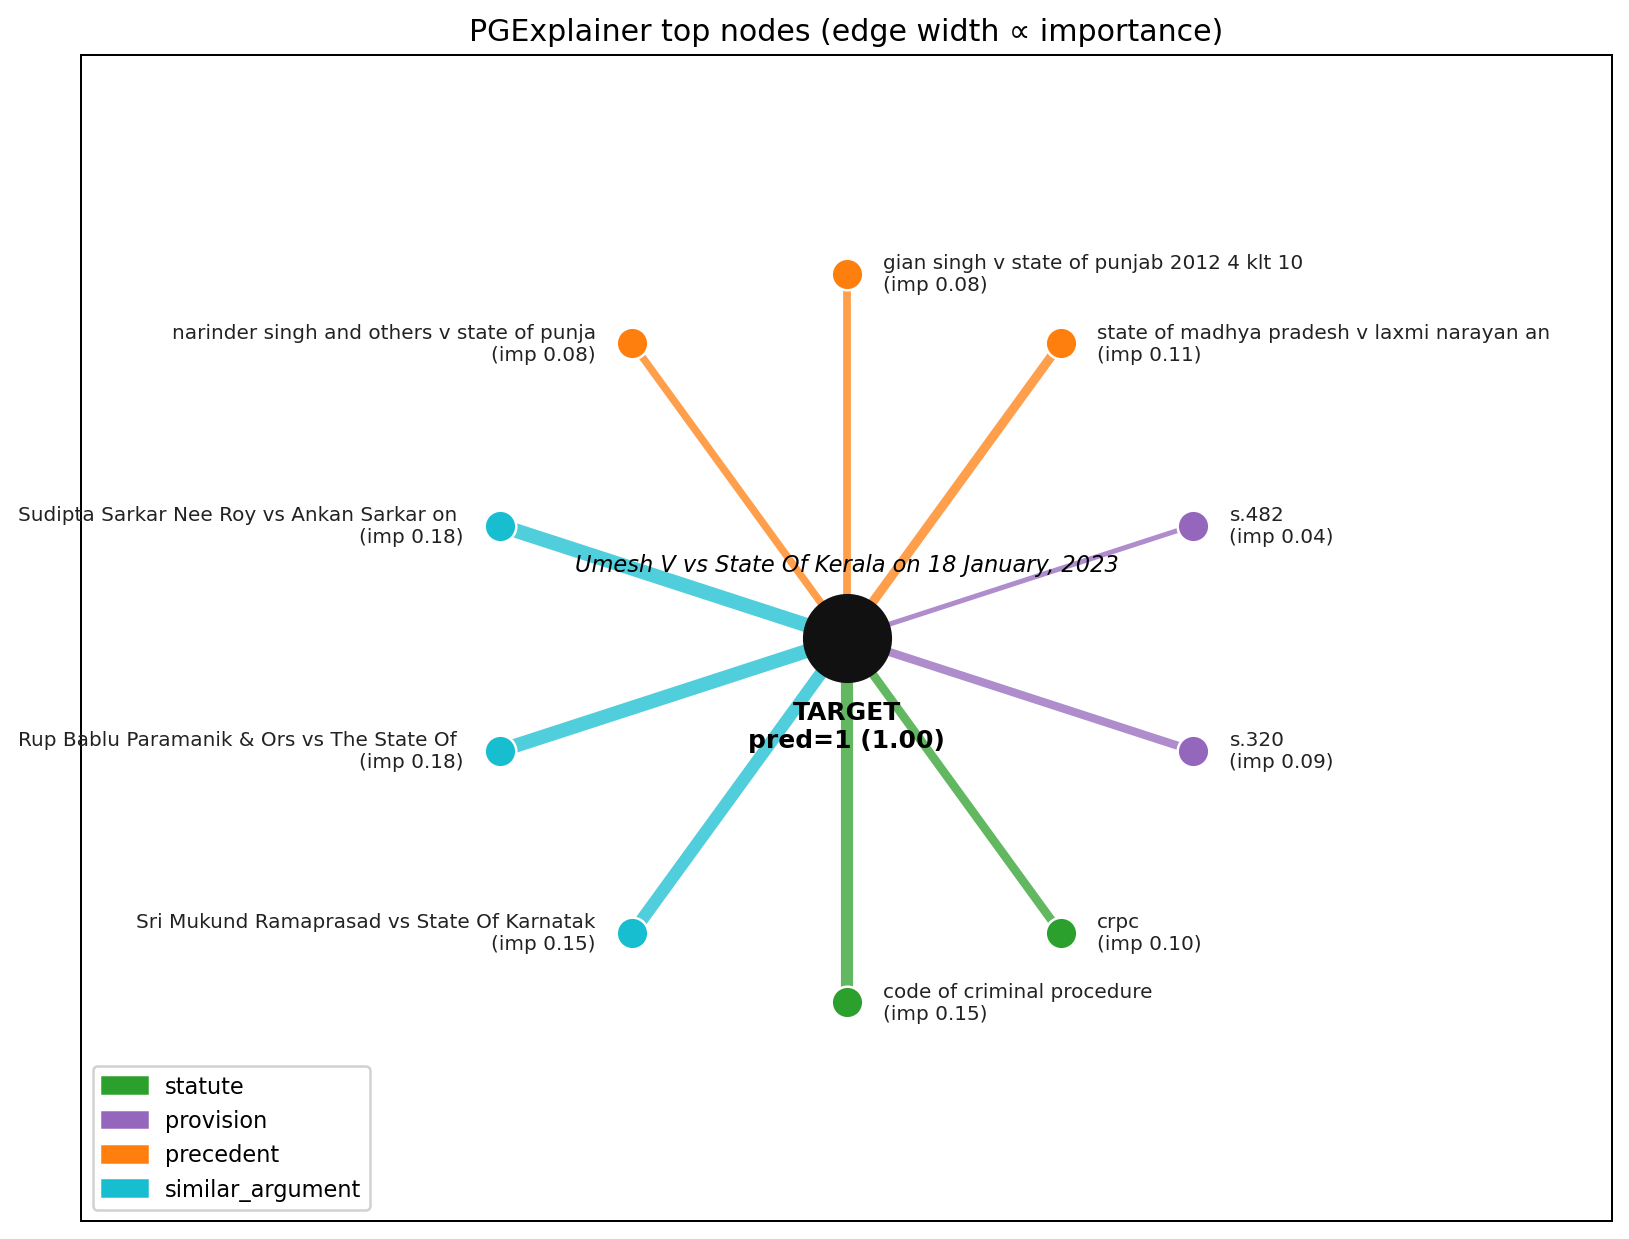
\includegraphics[width=\linewidth]{figures/explainability/wrong_13701_panel_b_subgraph.png}
  \end{minipage}
  \caption{Confidently-wrong case 13701. The target sits inside a dense cluster of structurally near-identical Kerala cases filed on the same day, all wins.}
  \label{fig:case_wrong}
\end{figure}

The evidence subgraph and the retrieved neighbours are not wrong in any local sense: the cases \emph{are} structurally close to the target in the model's representation. What the failure reveals is that a small number of distinguishing facts --- the specific factual configuration that led this court to refuse relief --- do not survive the embedding transformation. This is the structural signature of confident error on this corpus.

\section{Summary}

At the \emph{representation} level, the pre/post-GNN probe shows a $+3.97$-point gain attributable to message passing, and t-SNE shows the gain takes the form of within-domain outcome reorganisation. At the \emph{component} level, node-type zeroing and SHAP converge on the same story: the \textsc{Case} node dominates, but argument nodes and immediate participants contribute graph-local signal a plain text classifier cannot access. At the \emph{error} level, residual mistakes concentrate in doctrinally crowded cases, in fraud and sexual-offence buckets, and in the longest-facts quintile --- properties of the data, not of any model configuration. At the \emph{case} level, \path{Graph_Analyser} produces grounded, legally named explanations.

Crucially, the same pipeline exposes the model's \emph{confident} failure mode: for high-confidence predictions that are nevertheless wrong, top-$k$ retrieved neighbours overwhelmingly match the predicted (incorrect) label rather than the true one. A confident error is not an isolated mistake but a case placed inside the wrong outcome neighbourhood, whose explanation and prediction reinforce each other. Making that visible is what distinguishes a post-hoc explainer from a calibration metric.
